\documentclass{amsart}
\usepackage{tikz}
\usepackage{chessboard}
\author{David Prentiss}
\date{\today}
\title{Homework 1}
\begin{document}
\maketitle

\section{}
There are 6 teams in the football league: Vultures (V), Lions (L), Eagles (E),
Beavers (B), Terps (T) and Skunks (S).
The V's have already played the L's and the E's; the L's have also played the
B's \& S's.
The T's have played the E's and S's. Each team plays one game per week.
Find a schedule so that all teams will have played each other in the fewest
number of weeks.
Hint: Create a graph whose vertices are the pairs of teams that have not yet
played each other.
What should the edges be so that in a legal coloring of the graph each color can
represent the games played in one week?
Give a solution and show that it is optimal.

\subsubsection*{Solution}
$G = $
\begin{figure}[h]
  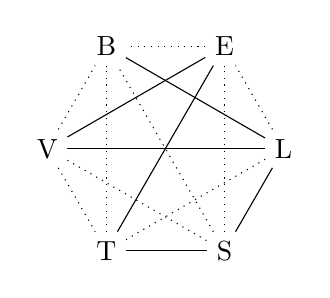
\begin{tikzpicture}
    \foreach [count=\i] \team in {B, E, L, S, T, V} {
      \node (\team) at (-60*\i+180:1.5cm) {\team};
    }
    \draw (T) -- (S);
    \draw (L) -- (B);
    \draw (V) -- (L);
    \draw (V) -- (E);
    \draw (L) -- (S);
    \draw (T) -- (E);
    \draw[dotted] (V) -- (B);
    \draw[dotted] (V) -- (T);
    \draw[dotted] (V) -- (S);
    \draw[dotted] (S) -- (E);
    \draw[dotted] (S) -- (B);
    \draw[dotted] (L) -- (T);
    \draw[dotted] (L) -- (E);
    \draw[dotted]  (T) -- (B);
    \draw[dotted]  (E) -- (B);
  \end{tikzpicture}
  \caption{A graph representing the league games thus far. A solid edge
    indicates the two teams have already played each other, while a dotted edge
    indicates a game between two teams that must be scheduled.}
\end{figure}

\section{}

(i) Show that in a nondirected graph G, the independence number of G  the dominance
number of G, by showing that every maximal independent set is a dominating set.
(ii) Give an example to show that the minimum dominating set is not necessarily
independent.

\section{}

Let $P_1$ and $P2$ be two paths in a graph $G$, and let $G^\prime=P_1 \bigcap P_2$ possess at least 2
vertices.
Show that if $G^\prime$ is disconnected then $P_1\bigcup P_2$ contains a cycle.

\section{}
A bipartite graph is given by the following adjacency list: a-1,2,5; b-1,3; c-2-3-5; d-4,5; e2,5,6; f-5,6.

\begin{figure}[h]
  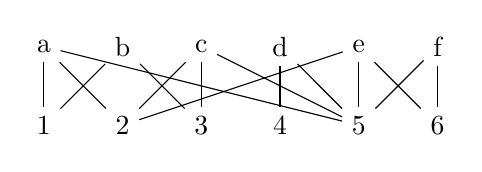
\begin{tikzpicture}
    \foreach [count=\i] \letter in {a, b, c, d, e, f} {
      \node (\letter) at (\i, 1) {\letter};
      \node (\i) at (\i, 0) {\i};
    }
    \draw (a) -- (1);
    \draw (a) -- (2);
    \draw (a) -- (5);
    \draw (b) -- (1);
    \draw (b) -- (3);
    \draw (c) -- (2);
    \draw (c) -- (3);
    \draw (c) -- (5);
    \draw (d) -- (4);
    \draw (d) -- (5);
    \draw (e) -- (2);
    \draw (e) -- (5);
    \draw (e) -- (6);
    \draw (f) -- (5);
    \draw (f) -- (6);
  \end{tikzpicture}
\end{figure}
\subsection*{a.}
Find the minimum vertex coloring. Prove that your solution is optimal.
\subsubsection*{Solution}
Let the above graph be graph $G$.
Since $G$ is bipartite, then by definition its vertices can be divided into two
disjoint sets such that no two edges in the same set are adjacent.
Since none of the edges in a set are adjacent, each set may be assigned a single
color and the graph will require at most two colors.
Therefore, since $G$ bipartite and not empty, it is 2-chromatic.
\begin{figure}[h]
  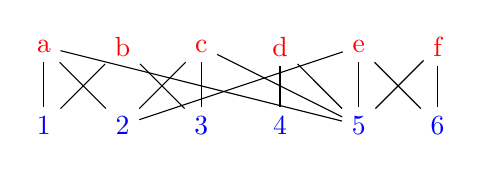
\begin{tikzpicture}
    \foreach [count=\i] \letter in {a, b, c, d, e, f} {
      \node[red] (\letter) at (\i, 1) {\letter};
      \node[blue] (\i) at (\i, 0) {\i};
    }
    \draw (a) -- (1);
    \draw (a) -- (2);
    \draw (a) -- (5);
    \draw (b) -- (1);
    \draw (b) -- (3);
    \draw (c) -- (2);
    \draw (c) -- (3);
    \draw (c) -- (5);
    \draw (d) -- (4);
    \draw (d) -- (5);
    \draw (e) -- (2);
    \draw (e) -- (5);
    \draw (e) -- (6);
    \draw (f) -- (5);
    \draw (f) -- (6);
  \end{tikzpicture}
\end{figure}

In a sense, $G$ is already two-colored in that the vertices $\{1,2,3,4,5,6\}$
are labeled with numerals while
$\{\text{a},\text{b},\text{c},\text{d},\text{e},\text{f}\}$
are labeled with letters.
However, while all bipartite graphs are 2-colorable, it is not the case that
they necessarily have a unique 2-coloring.
Consider $G$ for example, if the edge connecting nodes \{d\} and \{5\} were
removed, then the resulting subgraph containing \{d\} and \{4\} would
no longer be connected and we would have our choice of either coloring.
That is, (\{d\},\{4\}) or (\{4\},\{d\}).


\subsection*{b.}
Find the minimum edge coloring. What is a simple lower bound for the edge coloring of a
graph? Use this to prove that your solution is optimal.
\subsubsection*{Solution}
\begin{figure}[h]
  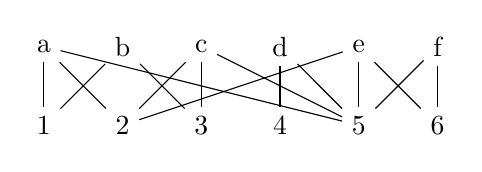
\begin{tikzpicture}
    \foreach [count=\i] \letter in {a, b, c, d, e, f} {
      \node (\letter) at (\i, 1) {\letter};
      \node (\i) at (\i, 0) {\i};
    }
    \draw (a) -- (1);
    \draw (a) -- (2);
    \draw (a) -- (5);
    \draw (b) -- (1);
    \draw (b) -- (3);
    \draw (c) -- (2);
    \draw (c) -- (3);
    \draw (c) -- (5);
    \draw (d) -- (4);
    \draw (d) -- (5);
    \draw (e) -- (2);
    \draw (e) -- (5);
    \draw (e) -- (6);
    \draw (f) -- (5);
    \draw (f) -- (6);
  \end{tikzpicture}
\end{figure}
\subsection*{c.}
Find a maximum matching. What is a simple upper bound to a maximum matching in a
graph? Use this to prove your solution is optimal.
\subsubsection*{Solution}
\begin{figure}[h]
  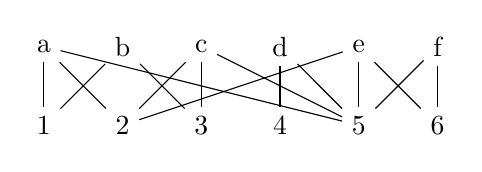
\begin{tikzpicture}
    \foreach [count=\i] \letter in {a, b, c, d, e, f} {
      \node (\letter) at (\i, 1) {\letter};
      \node (\i) at (\i, 0) {\i};
    }
    \draw (a) -- (1);
    \draw (a) -- (2);
    \draw (a) -- (5);
    \draw (b) -- (1);
    \draw (b) -- (3);
    \draw (c) -- (2);
    \draw (c) -- (3);
    \draw (c) -- (5);
    \draw (d) -- (4);
    \draw (d) -- (5);
    \draw (e) -- (2);
    \draw (e) -- (5);
    \draw (e) -- (6);
    \draw (f) -- (5);
    \draw (f) -- (6);
  \end{tikzpicture}
\end{figure}
\subsection*{d.}
Find a minimum edge cover. Prove that your solution is optimal.
\subsubsection*{Solution}
\begin{figure}[h]
  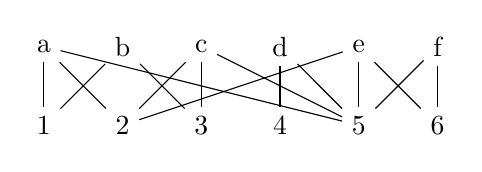
\begin{tikzpicture}
    \foreach [count=\i] \letter in {a, b, c, d, e, f} {
      \node (\letter) at (\i, 1) {\letter};
      \node (\i) at (\i, 0) {\i};
    }
    \draw (a) -- (1);
    \draw (a) -- (2);
    \draw (a) -- (5);
    \draw (b) -- (1);
    \draw (b) -- (3);
    \draw (c) -- (2);
    \draw (c) -- (3);
    \draw (c) -- (5);
    \draw (d) -- (4);
    \draw (d) -- (5);
    \draw (e) -- (2);
    \draw (e) -- (5);
    \draw (e) -- (6);
    \draw (f) -- (5);
    \draw (f) -- (6);
  \end{tikzpicture}
\end{figure}
\subsection*{e.}
Find a minimum vertex cover.
\subsubsection*{Solution}
\begin{figure}[h]
  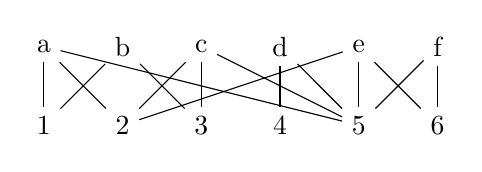
\begin{tikzpicture}
    \foreach [count=\i] \letter in {a, b, c, d, e, f} {
      \node (\letter) at (\i, 1) {\letter};
      \node (\i) at (\i, 0) {\i};
    }
    \draw (a) -- (1);
    \draw (a) -- (2);
    \draw (a) -- (5);
    \draw (b) -- (1);
    \draw (b) -- (3);
    \draw (c) -- (2);
    \draw (c) -- (3);
    \draw (c) -- (5);
    \draw (d) -- (4);
    \draw (d) -- (5);
    \draw (e) -- (2);
    \draw (e) -- (5);
    \draw (e) -- (6);
    \draw (f) -- (5);
    \draw (f) -- (6);
  \end{tikzpicture}
\end{figure}
\subsection*{f.}
Find a maximum independent set. Prove optimality of your solution.
\subsubsection*{Solution}
\begin{figure}[h]
  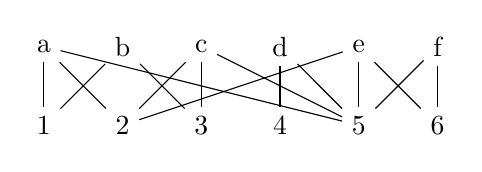
\begin{tikzpicture}
    \foreach [count=\i] \letter in {a, b, c, d, e, f} {
      \node (\letter) at (\i, 1) {\letter};
      \node (\i) at (\i, 0) {\i};
    }
    \draw (a) -- (1);
    \draw (a) -- (2);
    \draw (a) -- (5);
    \draw (b) -- (1);
    \draw (b) -- (3);
    \draw (c) -- (2);
    \draw (c) -- (3);
    \draw (c) -- (5);
    \draw (d) -- (4);
    \draw (d) -- (5);
    \draw (e) -- (2);
    \draw (e) -- (5);
    \draw (e) -- (6);
    \draw (f) -- (5);
    \draw (f) -- (6);
  \end{tikzpicture}
\end{figure}

\section{}
In a given connected graph with specified arc weights, suppose there exists an arc whose
weight is smaller than that of any other in G. Prove that this arc must be contained in every
minimum spanning tree in G.
\subsubsection*{Solution}

\section{}
Show that for any graph, $G$, the number of vertices with odd degree is even.
\begin{proof}
  Let $G=(V,E)$ have $k$ vertices. For every vertex, $v\in V$ exactly one of the
  following must be true.
  The degree of $v$, $\delta(v)$, must be either odd, even, or zero.
  Since this is true, we may partition the set of vertices in $G$, $V$, into
  three sets.
  Let $D\subseteq V$ be the set of vertices with odd degree,
  $N\subseteq V$ be the set of vertices with even degree,
  and $I\subseteq V$ be the set of vertices with zero degree.

  Now consider adding an edge, $e$, to the graph.
\end{proof}

\section{}
Is it possible for a cutset and a cycle to contain exactly one edge in common? Why?
\subsubsection*{Solution}

\section{}
Suppose forest $F$ consists of $t$ trees and contains $v$ vertices. How many
edges are in forest $F$?

\subsubsection*{Solution}

A forest $F$ of $t$ trees and $v$ vertices has $v-t$ edges.
\begin{proof}
\end{proof}

\section{} %9
A classic problem is the ``knight’s tour.''
On an $n \times n$ chessboard, starting from some
square, move the knight so that it lands on every space exactly once.
Show how a graph can be used to solve this problem.
Illustrate on a 4 by 4 chessboard.

\subsubsection*{Solution}
\begin{figure}[h]
  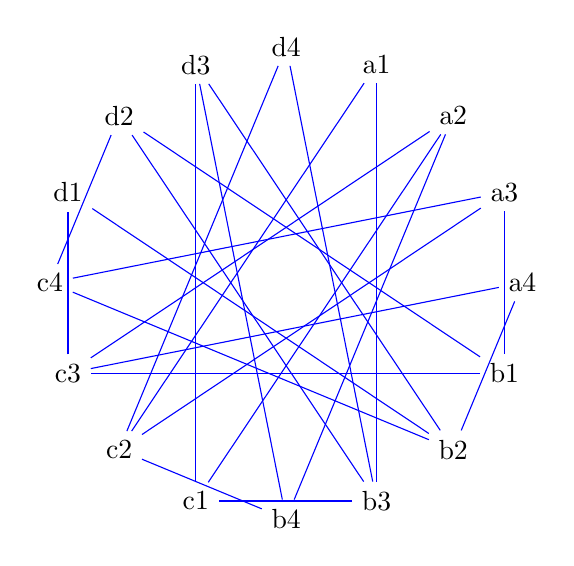
\begin{tikzpicture}
    \foreach [count=\i] \row in {1, 2, 3, 4} {
      \foreach [count=\j] \col in {a, b, c, d} {
       \node (\col\row) at ({-360/16*(\i+(4*\j))+180}:3cm) {\col\row};
      }
    }
    \draw[blue] (a1) -- (c2);
    \draw[blue] (a1) -- (b3);
    \draw[blue] (c2) -- (a3);
    \draw[blue] (c2) -- (b4);
    \draw[blue] (c2) -- (d4);
    \draw[blue] (b3) -- (d4);
    \draw[blue] (b3) -- (d2);
    \draw[blue] (b3) -- (c1);
    \draw[blue] (a3) -- (b1);
    \draw[blue] (a3) -- (c4);
    \draw[blue] (b4) -- (a2);
    \draw[blue] (b4) -- (d3);
    \draw[blue] (d2) -- (b1);
    \draw[blue] (d2) -- (c4);
    \draw[blue] (c1) -- (a2);
    \draw[blue] (c1) -- (d3);
    \draw[blue] (b1) -- (c3);
    \draw[blue] (c4) -- (b2);
    \draw[blue] (a2) -- (c3);
    \draw[blue] (d3) -- (b2);
    \draw[blue] (c3) -- (a4);
    \draw[blue] (c3) -- (d1);
    \draw[blue] (b2) -- (a4);
    \draw[blue] (b2) -- (d1);
  \end{tikzpicture}
  \caption{}
\end{figure}


\begin{figure}[h]
\chessboard[
maxfield=d4,
showmover=false
]
  \caption{}
\end{figure}


\section{}
Show how to use a graph to solve the following puzzle. Place the numbers 1 through 8 in the
boxes so that no two consecutive numbers are horizontally, vertically, or diagonally adjacent
to each other.
\subsubsection*{Solution}

\section{}
Using big O notation, given the worst-case running times of the following four procedures
as a function of $n$.
\subsubsection*{Solution}


\end{document}

\begin{tikzpicture}
  \graph [circular placement, nodes={draw, circle}] {
    V -- {L, E}; L -- {B, S}; T -- {E, S};
  };
\end{tikzpicture}

    \draw[blue] (a1) -- (c2);
    \draw[blue] (a1) -- (b3);
    \draw[blue] (c2) -- (a3);
    \draw[blue] (c2) -- (b4);
    \draw[blue] (c2) -- (d4);
    \draw[blue] (b3) -- (d4);
    \draw[blue] (b3) -- (d2);
    \draw[blue] (b3) -- (c1);
    \draw[blue] (a3) -- (b1);
    \draw[blue] (a3) -- (c4);
    \draw[blue] (b4) -- (a2);
    \draw[blue] (b4) -- (d3);
    \draw[blue] (d2) -- (b1);
    \draw[blue] (d2) -- (c4);
    \draw[blue] (c1) -- (a2);
    \draw[blue] (c1) -- (d3);
    \draw[blue] (b1) -- (c3);
    \draw[blue] (c4) -- (b2);
    \draw[blue] (a2) -- (c3);
    \draw[blue] (a2) -- (c3);
    \draw[blue] (d3) -- (b2);